
The input sequence of embeddings
$\mathbf{x} \in \mathbb{R}^{n \times d_{\text{model}}}$ is passed into the first encoder block all at once, and the output of that block is then passed through the next transformer block until the sequence has been passed through all $L = 12$ blocks. The final output of the encoder is the encoded representation of $\mathbf{x}$. (\cite{thickstun_transformer_2020})

An encoder block can therefore be thought of as a function $f: \mathbb{R}^{n \times d_{\text{model}}} \rightarrow \mathbb{R}^{n \times d_{\text{model}}}$
where $f(\mathbf{x}) = \mathbf{z} \in \mathbb{R}^{n \times d_{\text{model}}}$, and the encoder can be thought of as composition $f_L \circ f_{L-1} \circ \dots \circ f_1$. (\cite{thickstun_transformer_2020})

This can also be illustrated by the diagram:

\begin{figure}[H]
    \centering
    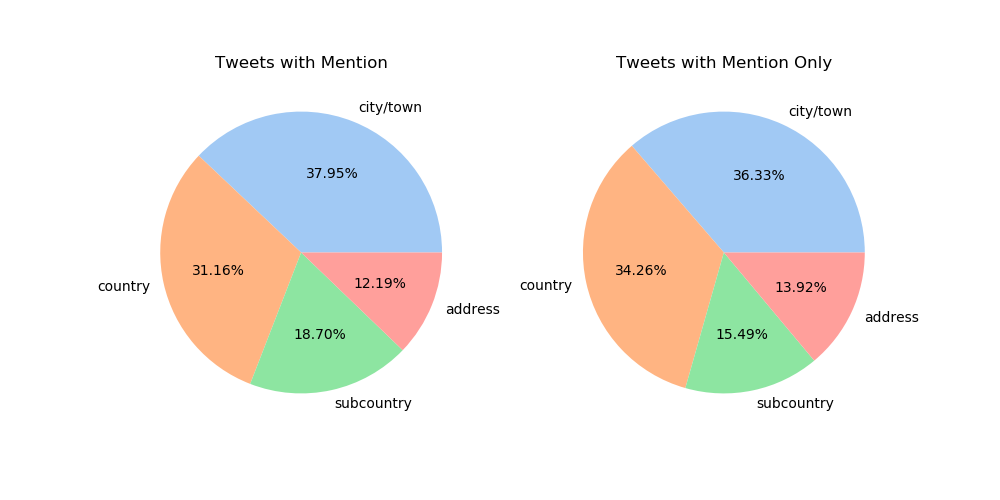
\includegraphics[width=0.5\textwidth]{images/mention_pie.png}
    \caption{Transformer Block}
    \label{fig:transformer-block}
\end{figure}

Each encoding transformer block consists of a stack of multiple identical transformer blocks, each of which consists of two sub-layers: a multi-head self-attention layer (MHA) and a position-wise feedforward network (FFN). \cite{vaswani_attention_2017}

The function $f$ can be written as:

$$f(\mathbf{x}) = \mathbf{z}$$
\begin{equation} \label{sublayer1}
    \mathbf{u}= \text{LayerNorm}(\mathbf{\mathbf{x}} + \text{MHA}(\mathbf{x}))
\end{equation}
\begin{equation} \label{sublayer2}
    \mathbf{z} = \text{LayerNorm}(\mathbf{u} + \text{FFN}(\mathbf{\mathbf{u}}))
\end{equation}

\subsection{Multi-Head Attention}

\subsubsection{What is attention?}
The attention mechanism enables neural networks to assign varying degrees of importance or attention to individual elements within a sequence. "Self" in self-attention refers to the fact that the computation of attention weights is performed based on the hidden states of the same sequence rather than using external context or information from another sequence. 
Self-attention involves using the entire sequence to determine the weight of each token's embedding rather than assigning a fixed embedding to each token. In other words, self-attention generates a new sequence of embeddings ($y_1, \dots, y_n$) based on a given sequence of token embeddings ($x_1, \dots, x_n$). Each new embedding $y_i$ is a weighted sum of all the token embeddings $x_j$, where the attention weights $w_{ij}$ are normalized such that $\sum_{}^{} w_{i,j} = 1$. (\cite{tunstall_natural_2022})
$$y_i = \sum_{j=1}^{n} w_{i,j} x_j$$
In the "duck" example, without context, the word might refer to a type of bird. However, with additional context, such as "I saw her duck to hide," it is clear that it pertains to the verb. To create a representation of "duck" that captures this context, all the token embeddings can be blended in various proportions by assigning greater weights $w_{ij}$ to the embeddings for "to" and "hide." These embeddings produced through this process are referred to as contextualized embeddings.

In BERT's multi-head attention layer, the attention mechanism is called "scaled dot-product attention" and is applied $A = 12$ times to the input sequence in parallel. (\cite{tunstall_natural_2022})


\subsubsection{Scaled Dot-Product Attention}

The input
$\mathbf{x} \in \mathbb{R}^
{n \times d_{\text{model}}}$
is first multiplied by projection matrices
$\mathbf{W}^Q, \mathbf{W}^K \in \mathbb{R}^
{d_{\text{model}} \times d_{\text{k}}}$
,
$\mathbf{W}^V \in \mathbb{R}^
{d_{\text{model}} \times d_{\text{v}}}$
to get the query, key and value matrices:
$ \mathbf{W}^Q \mathbf{x} = \mathbf{Q} \in \mathbb{R}^
{n \times d_{\text{k}}}$, 
$ \mathbf{W}^K  \mathbf{x} = \mathbf{K} \in \mathbb{R}^
{n \times d_{\text{k}}}$, 
$ \mathbf{W}^V \mathbf{x} = \mathbf{V} \in \mathbb{R}^
{n \times d_{\text{v}}}$. (\cite{thickstun_transformer_2020})
Note that each row in $\mathbf{x}$ is an embedding for each of the $n$ tokens in the sequence. By multiplying by $\mathbf{W}^Q, \mathbf{W}^K, \mathbf{W}^V$, each embedding vector is projected into three vectors (known as query, key and value) (\cite{tunstall_natural_2022}).

The attention scores are calculated using a similarity function, which is the "dot product." This is done by multiplying matrices $\mathbf{Q}\mathbf{K}^T \in \mathbb{R}^
{n \times n}$, which corresponds to attention scores for each token $n$. (\cite{tunstall_natural_2022})

The attention scores are multiplied by a scaling factor $d_{\text{k}}$ to smooth gradients during training by normalizing their variance (\cite{geron_hands-machine_2019}). Then the result is passed through the softmax function \cite{geron_hands-machine_2019}, so all column values sum to 1 to get the attention weights:
$$\text{softmax}(\frac{\mathbf{Q}\mathbf{K}^T}{\sqrt{d_k}}) \in  \mathbb{R}^
{n \times n}$$

For a given input matrix $X$ of shape $(m, n)$, where m is the number of rows and n is the number of columns, the softmax function \cite{geron_hands-machine_2019} is defined as:

$$ \mathrm{softmax}(X_{i,j}) = \frac{e^{X_{i,j}}}{\sum_{k=1}^m e^{X_{k,j}}} $$

where $i$ is the row index and $j$ is the column index.


\begin{figure}[H]
    \centering
    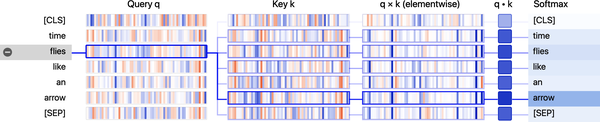
\includegraphics[width=1\textwidth]{images/QKV.png}
    \caption{Visualisation of Attention Mechanism}
    \label{fig:attention}
\end{figure}

The attention weights are multiplied by the values matrix to complete the scaled dot-product attention step (\cite{tunstall_natural_2022}). This results in an updated representation of each embedding:

\begin{align*}
    Attention(\mathbf{Q}, \mathbf{K}, \mathbf{V}) = softmax(\frac{\mathbf{Q}\mathbf{K}^T}{\sqrt{d_k}})\mathbf{V}
\end{align*}

This step can be summarised in terms of equations by:

$$ \mathbf{Q} = \mathbf{W}^Q \mathbf{x} \in \mathbb{R}^
{n \times d_{\text{k}}}$$
$$ \mathbf{K} = \mathbf{W}^K  \mathbf{x} \in \mathbb{R}^
{n \times d_{\text{k}}}$$
$$ \mathbf{V} = \mathbf{W}^V \mathbf{x} \in \mathbb{R}^
{n \times d_{\text{v}}}$$

\begin{align*}
    \text{head} = Attention(\mathbf{Q}, \mathbf{K}, \mathbf{V}) = softmax(\frac{\mathbf{Q}\mathbf{K}^T}{\sqrt{d_k}})\mathbf{V}
\end{align*}

\subsubsection{Multi-Head Attention}

Multi-head attention is a variant of scaled dot-product attention that splits the input into multiple "heads" and computes the attention for each head separately (\cite{tunstall_natural_2022}). So for each head $ a = 1, \dots, A$:

\begin{align*}
    \text{head}_a = Attention(\mathbf{Q}_a, \mathbf{K}_a, \mathbf{V}_a) = softmax(\frac{\mathbf{Q}_{a}\mathbf{K}_{a}^T}{\sqrt{d_k}})\mathbf{V}_a
\end{align*}

where 
$$ \mathbf{Q}_a = \mathbf{W}_a^Q \mathbf{x} \in \mathbb{R}^
{n \times d_{\text{k}}}$$
$$ \mathbf{K}_a = \mathbf{W}_a^K \mathbf{x} \in \mathbb{R}^
{n \times d_{\text{k}}}$$
$$ \mathbf{V}_a = \mathbf{W}_a^\mathbf{V} \mathbf{x} \in \mathbb{R}^
{n \times d_{\text{v}}}$$

Then outputs of $\text{head}_a$ are concatenated and projected using $\mathbf{W}^O \in \mathbb{R}^
{Ad_v \times d_{\text{model}}}$ (\cite{vaswani_attention_2017}).

\begin{align*}
    MHA(\mathbf{Q}, \mathbf{K}, \mathbf{V}) = \text{Concat}(\text{head}_1, \dots, \text{head}_A)\mathbf{W}^O
\end{align*}

Remember, by definition $d_v = d_\text{model}/A = 64$, so  $\mathbf{u} = MHA(\mathbf{Q}, \mathbf{K}, \mathbf{V}) \in \mathbb{R}^
{n \times d_{\text{model}}}$.

Note that the projection matrices $\mathbf{W}_a^Q$, $\mathbf{W}_a^K$, $\mathbf{W}_a^V$, $\mathbf{W}^O$ are learnable projection matrices. For now, assume they work. How they are learned is discussed in Section %\ref{gradient-descent}.

\subsection{Layer Normalisation 1}

Remember that the output of the first sublayer of the encoder block (\ref{sublayer1}) contains a residual connection, i.e., the original output $\mathbf{x}$ is added to the output of the MHA layer. The resulting sum is then passed through a layer normalization step. This "Add \& Norm" layer can be mathematically represented (\cite{thickstun_transformer_2020}) as:

$$\text{AddNorm}(\mathbf{x}) = \text{LayerNorm}(\mathbf{x} + \text{MHA}(\mathbf{x}); \alpha_1, \beta_1)$$

For a given input matrix $ X \in \mathbb{R}^
{n \times m}$, the layer normalization function is defined as:

\begin{equation} \label{layernorm}
    \mathrm{LayerNorm}(X_{i}) = \alpha_1\frac{X_{i} - \mu_i}{\sqrt{\sigma_i^2 + \epsilon}} + \beta_1 
\end{equation}

$$\mu_i = \frac{1}{n}\sum_{j=1}^n X_{i,j}$$

$$\sigma_i = \sqrt{\frac{1}{n}\sum_{j=1}^n (X_{i,j}-\mu_i)^2}$$

where $i$ is the row index, $\mu_i$ is the mean of the $i$-th row, $\sigma_i$ is the standard deviation of the $i$-th row (\cite{thickstun_transformer_2020}), and $\epsilon$ is a small constant added to avoid division by zero (\cite{huang_annotated_2022}), $\alpha_1, \beta_1 \in \mathbb{R}^{n}$ are learned parameters (\cite{thickstun_transformer_2020}).

Residual connections and layer normalization help alleviate the vanishing gradient problem and improve the stability of the training process. (\cite{vaswani_attention_2017})

\subsection{Feed-Forward Network}

Moving onto the second sublayer (\ref{sublayer2}).
The position-wise feedforward network consists of two linear transformations with a ReLU activation function in between, which enables the model to capture complex non-linear relationships between the input sequence and the output embeddings.

The feedforward sublayer of the Transformer block takes the output of the MHA sublayer and applies a two-layer fully connected neural network to each token in the input sequence. The feedforward sublayer can be mathematically represented (\cite{vaswani_attention_2017}) as follows:

\begin{equation}
    \text{FFN}(\mathbf{x}) = \text{ReLU}(\mathbf{x} \mathbf{W}_1 + \mathbf{b}_1) \mathbf{W}_2 + \mathbf{b}_2 
     = \max(0, \mathbf{x} \mathbf{W}_1 + \mathbf{b}_1) \mathbf{W}_2 + \mathbf{b}_2
\end{equation}

where $\mathbf{x}$ is the output of the self-attention sublayer, $\mathbf{W}_1 \in \mathbb{R}^
{d_{\text{model}} \times d_{ff}}$ and $\mathbf{W}_2 \in \mathbb{R}^{d_{ff} \times d_{\text{model}}}$ are learnable weight matrices for the first and second layers of the fully connected network, respectively, and $\mathbf{b}_1 \in \mathbb{R}^{d_{ff}}$ and $\mathbf{b}_2 \in \mathbb{R}^{d_{\text{model}}}$ are learnable bias vectors for the first and second layers, respectively. $d_{ff}$ is the inner layer dimensionality, and in BERT $d_{ff} = 4d_\text{model} = 3072$.

\subsection{Layer Normalisation 2}

The output of the feedforward sublayer is then passed through another "Add \& Norm" sublayer, which can be mathematically represented as \cite{thickstun_transformer_2020}:

$$\text{AddNorm}(\mathbf{u}) = \text{LayerNorm}(\mathbf{u} + \text{FFN}(\mathbf{u}); \alpha_2, \beta_2)$$

\subsection{Summary of Transformer Block}

BERT has $L = 12$ encoder blocks, each of which can be defined as a function $f_l(\mathbf{x}) = z \in \mathbb{R}^{n \times d_{\text{model}}}$ where:
$$f_l(\mathbf{x}) = \mathbf{z}$$
\begin{equation}
    \mathbf{u}= \text{LayerNorm}(\mathbf{\mathbf{x}} + \text{MHA}(\mathbf{x}); \alpha_1, \beta_1)
\end{equation}
\begin{equation} 
    \mathbf{z} = \text{LayerNorm}(\mathbf{u} + \text{FFN}(\mathbf{\mathbf{u}}); \alpha_2, \beta_2)
\end{equation}
where MHA is defined as:
\begin{align*}
    \text{MHA}(\mathbf{Q}, \mathbf{K}, \mathbf{V}) = \text{Concat}(head_1, \dots, head_A)\mathbf{W}^O
\end{align*}
\begin{align*}
    \text{head}_a = \text{Attention}(\mathbf{Q}_a, \mathbf{K}_a, \mathbf{V}_a) = \text{softmax}(\frac{\mathbf{Q}_{a}\mathbf{K}_{a}^T}{\sqrt{d_k}})\mathbf{V}_a
\end{align*}
$$ \mathbf{Q}_a = \mathbf{W}_a^Q  \mathbf{x} \in \mathbb{R}^
{n \times d_{\text{k}}}$$
$$ \mathbf{K}_a = \mathbf{W}_a^K \mathbf{x} \in \mathbb{R}^
{n \times d_{\text{k}}}$$
$$ \mathbf{V}_a = \mathbf{W}_a^\mathbf{V}  \mathbf{x} \in \mathbb{R}^
{n \times d_{\text{v}}}$$

and FFN is defined as: 
$$\text{FFN}(\mathbf{x}) = \max(0, \mathbf{x} \mathbf{\mathbf{W}}_1 + \mathbf{b}_1) \mathbf{W}_2 + \mathbf{b}_2$$
The learnable parameters of the encoder block are shown in Table \ref{tab:bert-parameters}.

\begingroup
\setlength{\tabcolsep}{10pt} % Default value: 6pt
\renewcommand{\arraystretch}{1.5} % Default value: 1
\begin{table}[H]
\centering
    \begin{tabular}{c|c|c}
    \textbf{Layer} & \textbf{Parameters} & \textbf{Dimensions} \\ \hline
     MHA & $\mathbf{W}_a^Q, \mathbf{W}_a^K$ & $\mathbb{R}^{d_{\text{model}} \times d_{\text{k}}}$ \\
    
    & $\mathbf{W}_a^V$ & $\mathbb{R}^{d_{\text{model}} \times d_{\text{v}}}$ \\
    
    & $\mathbf{W}^O$ & $\mathbb{R}^{Ad_v \times d_{\text{model}}}$ \\ \hline
     
     FFN & $\mathbf{W}_1$ & $\mathbb{R}^{d_{\text{model}} \times d_{ff}}$ \\
     & $\mathbf{W}_2$ & $\mathbb{R}^{d_{ff} \times d_{\text{model}}}$ \\
     & $\mathbf{b}_1$ & $\mathbb{R}^{d_{ff}}$ \\
     & $\mathbf{b}_2$ & $\mathbb{R}^{d_{\text{model}}}$ \\ \hline
     
    LayerNorm & $\alpha_1, \beta_1$ & $\mathbb{R}^n$ \\
     & $\alpha_2, \beta_2$ & $\mathbb{R}^n$ \\ 
    \end{tabular}
\caption{Learnable Parameters of Encoder Block}
\label{tab:bert-parameters}
\end{table}
\endgroup


